\chapter{Robot Helper} % Main chapter title

\label{chapter:plan_management} % Change X to a consecutive number; for referencing this chapter elsewhere, use \ref{ChapterX}

\lhead{Chapter 4. \emph{Plan Production and Management}} % Change X to a consecutive number; this is for the header on each page - perhaps a shortened title


\section{Robot Helper}
\label{sec:case_study-helper}
\subsection{Introduction}
\label{subsec:case_study-helper-intro}
In this section we show experiments created to validate our system in a domestic scenario, where the robot can help a human partner to achieve a joint task. Parts of this section were presented in \cite{fioreiser2014}.

\subsection{Experiment Description}
We present a scenario where the robot and a human have a joint goal: cleaning a set of furniture. 
The environment is composed by two different furniture, a $TABLE$ and a $SHELF$, and three tapes,
 $TAPE1$, $TAPE2$ and $TAPE3$. The goal of the agents is throwing each tape in a $BIN$. We will present different examples, where the items will be placed differently, depending on our needs. The scenario is shown in figure \ref{fig:case_study-helper-pr2helper}

 \begin{figure}[ht!]
 	\centering
 	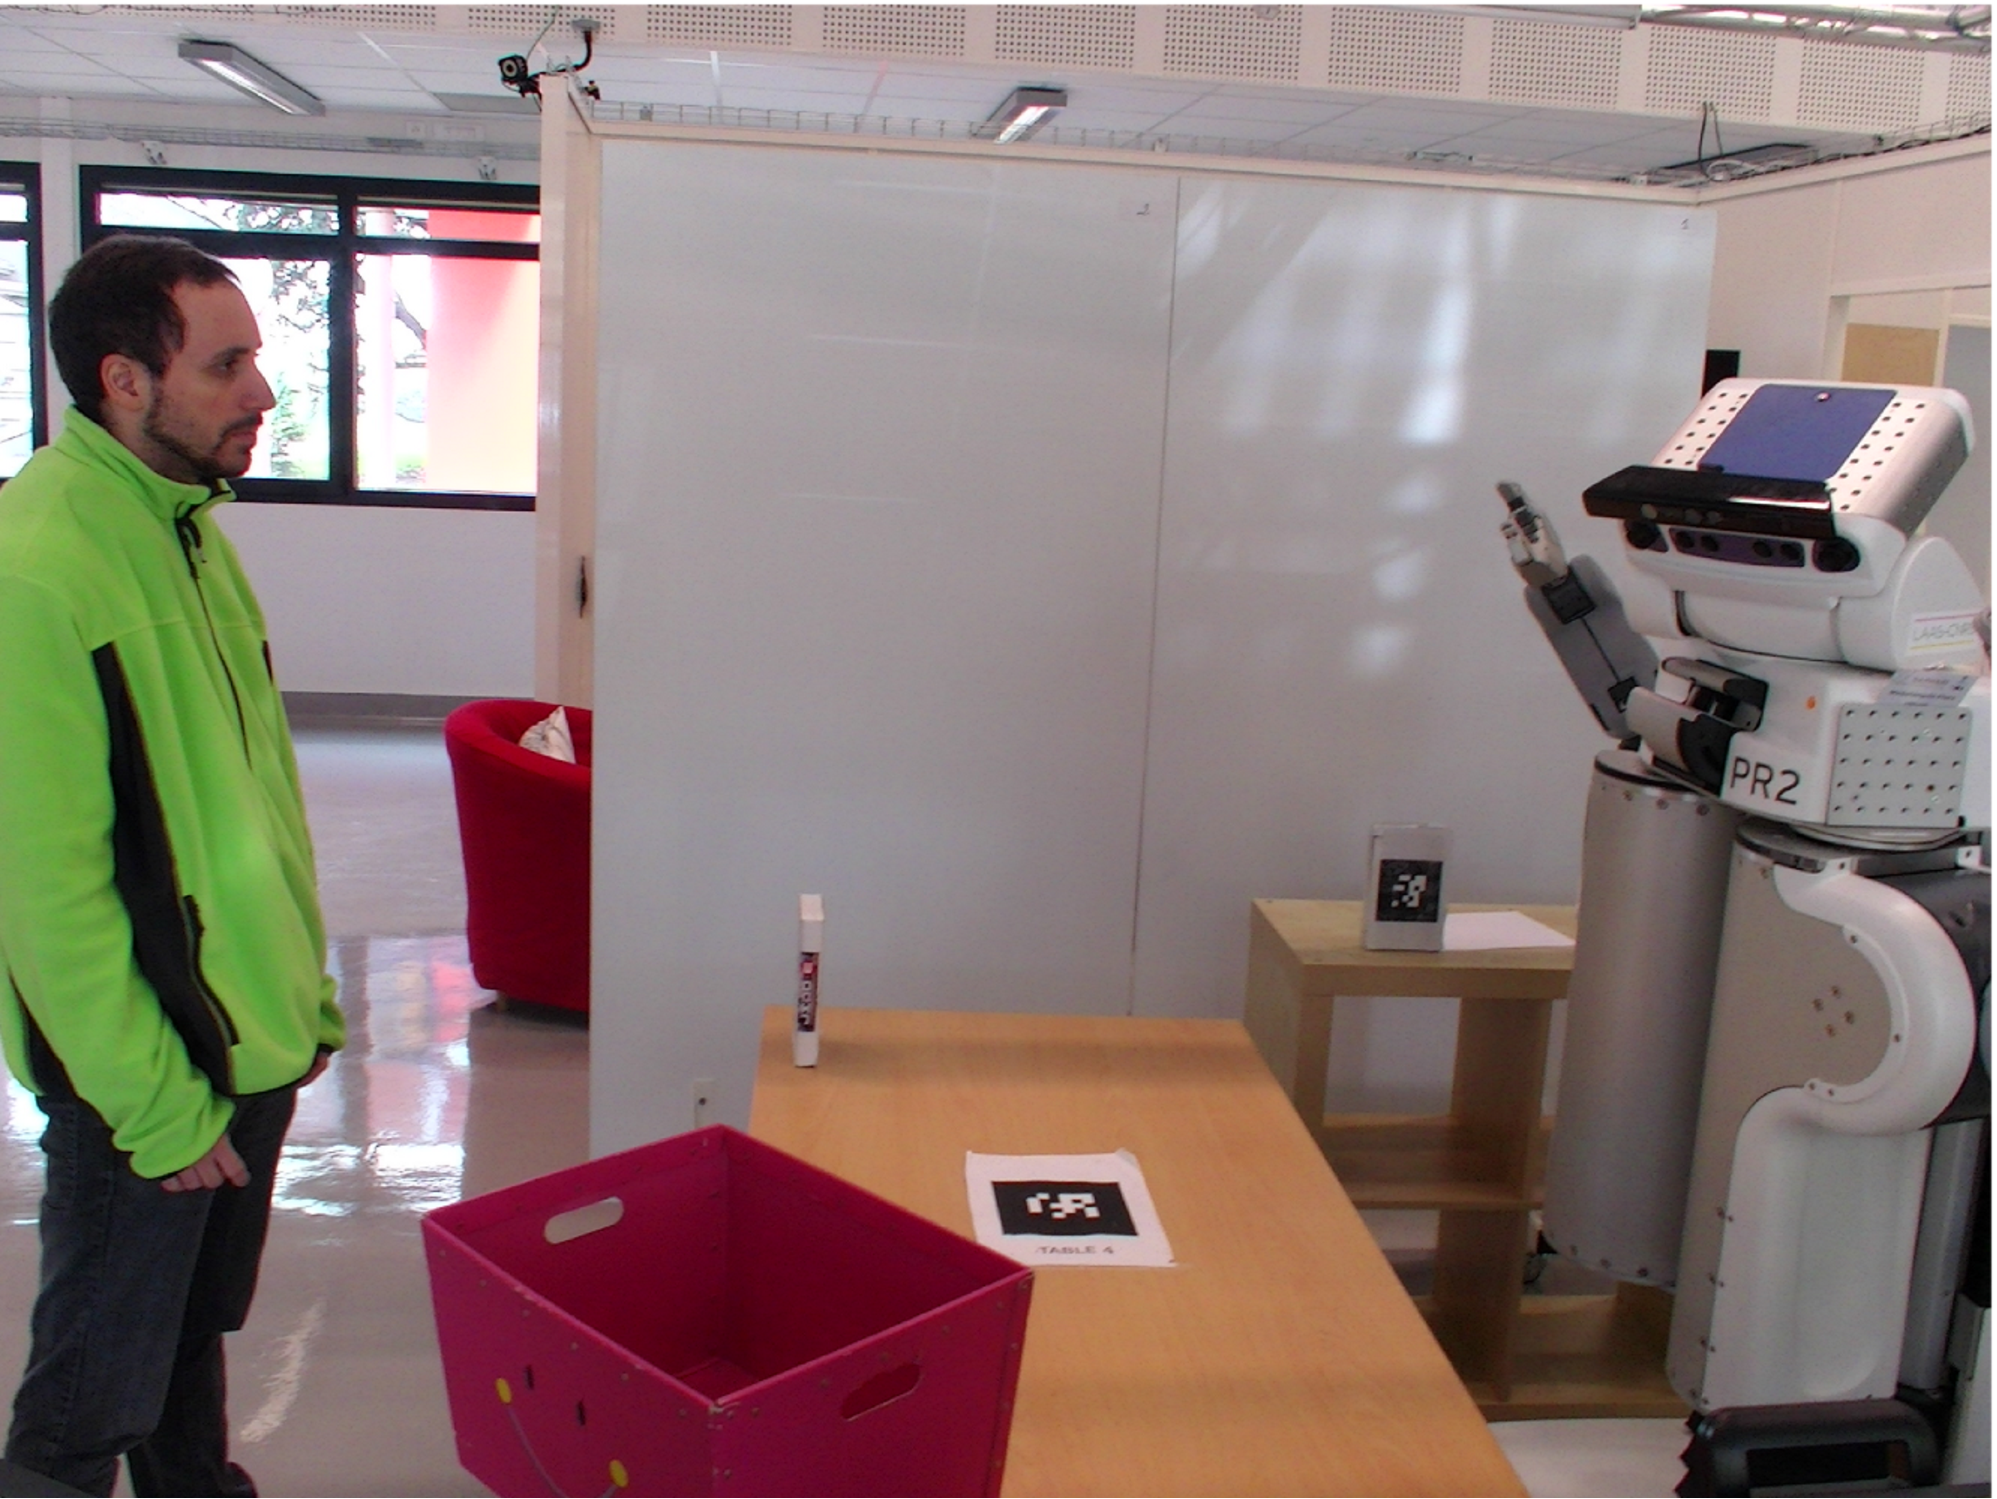
\includegraphics[scale=0.45]{img/case_study/helper/experiment.pdf}
 	\caption{The robot helper scenario, with a PR2 robot and a user.}
 	\label{fig:case_study-helper-pr2helper}
 \end{figure}

For this scenario, we used a previous version of our system, with the addition of the Handover Collaboration Planner, used to execute human-robot and robot-human handovers. In particular, in this version, the robot does not take into account the knowledge level of users when producing or managing plans. Also, human tracking will be done using a depth camera, mounted on the ceiling.

\subsection{Handover Collaboration Planner}
\label{subsec:case_study-helper-handover}
We implemented a MOMDP model to handle handovers between humans and robots. This model will output high-level actions, adapted by the Action Executor, depending on the current situation. Decisions will be made based on the following variables:

\begin{itemize}
\item The status of advancement of the task. This variables, whose values are \textit{\{not\_completed, touching, completed\}}, is set by the Action Executor module, in the Execution Management layer, depending on the current advancement of the task. The variable will be set as $completed$ when the handover has been performed, $touching$ when the robot detects pressure on the gripper used for the handover, and $not\_completed$ otherwise. 
\item The quality of commitment of the user. This variable has the same meaning as in the collaborative planner for guiding presented in \ref{subsec:case_study-spencer-collaborative_guide_planner} and can assume the same values, but is estimated from different variables. We will still consider the distance and orientation of the human toward the robot, but also the pose of its arm, particularly if its extended toward the robot. 
\item A timer. The variable is used in the same way as in the collaborative planner for guiding, presented in subsection~\ref{subsec:case_study-spencer-collaborative_guide_planner}.
\end{itemize}

The possible actions of this model are the following:
\begin{itemize}
\item Continue. The Action Executor will continue with the handover, which, depending on the situation, will prompt the system to extend the arm or activate the gripper.
\item Wait. The system will wait for the user if he is not engaged in the task.
\item Abandon. The system will abandon the task when the user is no longer interested in performing it. 
\end{itemize} 

\subsection{Experiments}
\label{subsec:case_study-helper-experiments}
We will describe different experiments conducted in our laboratory.

\begin{itemize}
  \item
\textbf{Equal Partners}:
In this scenario (figure \ref{fig:case_study-helper-scenario1}) the user is asked to clean the table, without explaining him what is the shared plan that will be used. The user is just informed that
the robot will try to help as it can to perform the task. The user moves to the table and
takes the \textit{TAPE2}. At this point, the robot notices that the user
has completed an action and understands that he wants to clean the
table.
\begin{figure}
  \caption[Robot helper experiment 1]{Robot adapts. This figure shows the robot's representation of the scenario. The white tape is the \textit{TAPE2}, while the blue
    one is the \textit{TAPE1}. The round shapes represent the agents'
    rechabilities, with red shapes representing robot reachabilities
    and green shapes human reachabilities. In this case only the human
  can reach the \textit{TAPE2} while both agents can reach the \textit{TAPE1}
and the \textit{BIN}. After the human takes the \textit{TAPE2} the
robot produces a plan where the human must throw the tape in the
bin while the robot can take the \textit{TAPE1} and throw it in the
bin.
}
\centering
  \subfigure{
  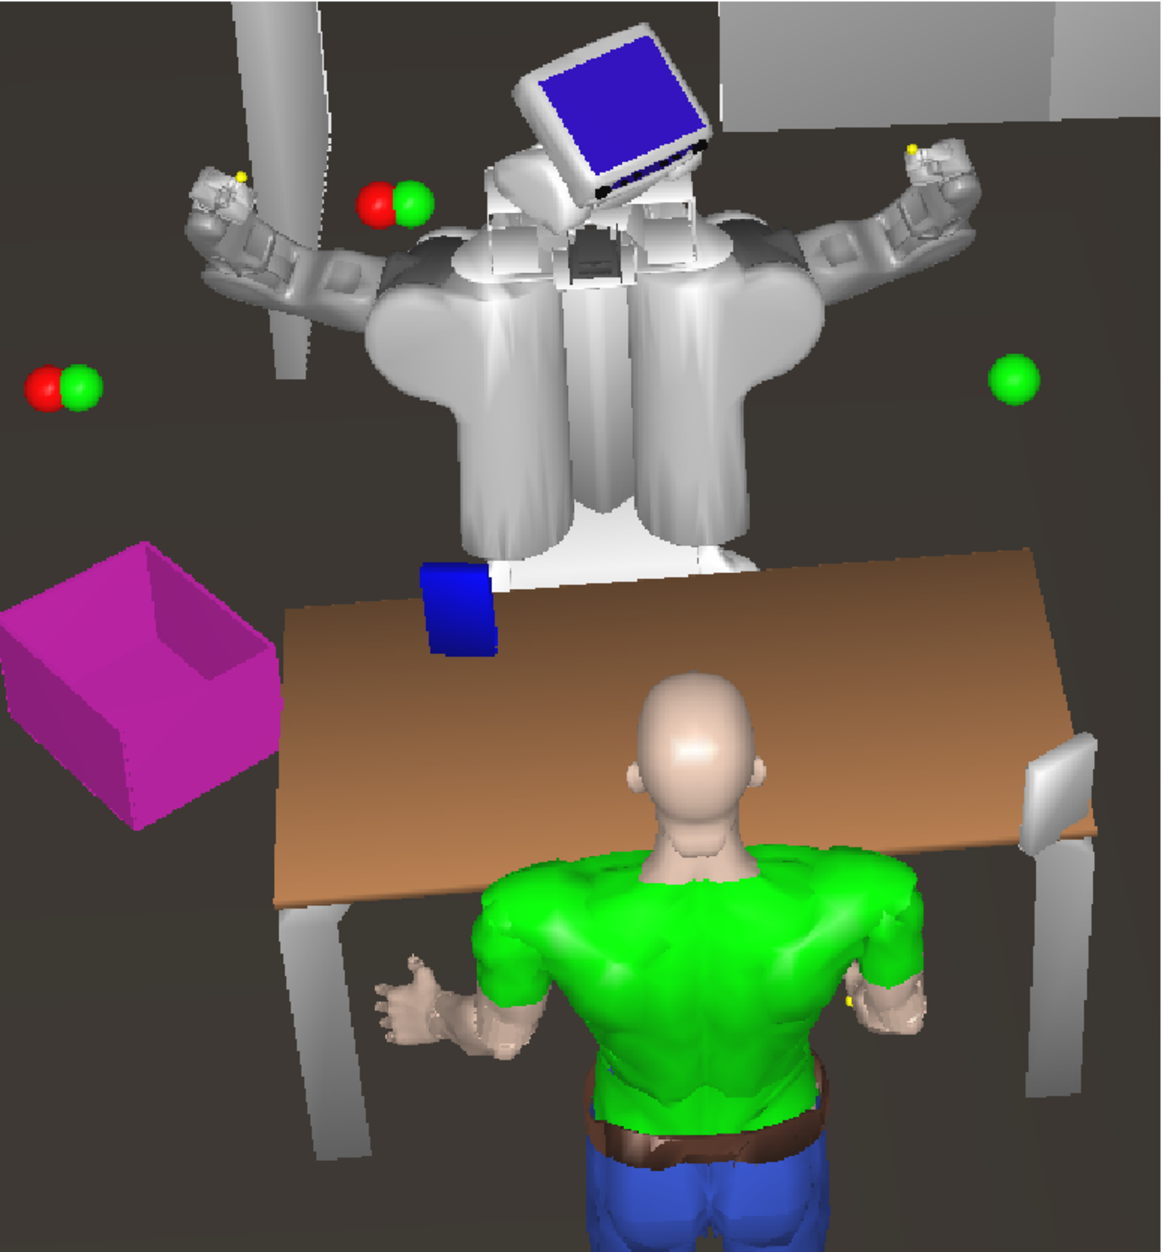
\includegraphics[scale=0.25]{img/case_study/helper/scenario1.pdf}
  }
  \subfigure{
  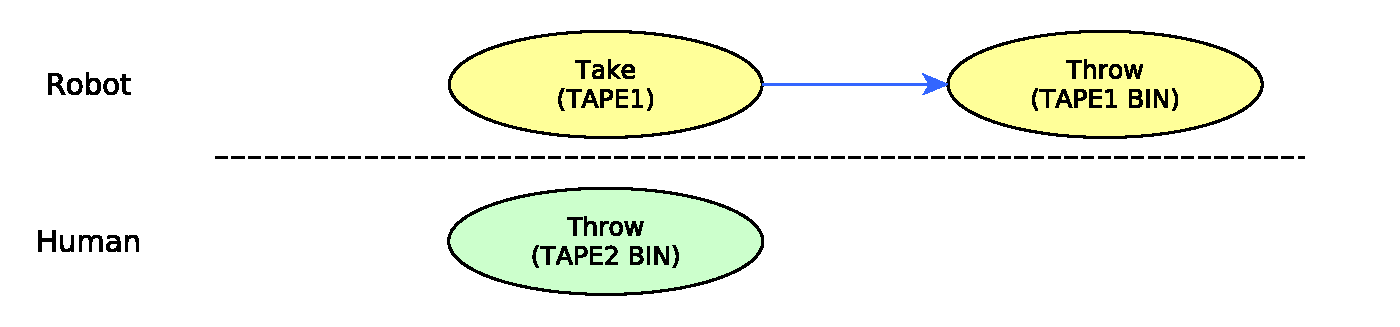
\includegraphics[scale=0.7]{img/case_study/helper/plan1.pdf}
  }
  \label{fig:case_study-helper-scenario1}
\end{figure}

The robot creates a plan and executes its part of it while monitoring the human,
which executes its part without deviating from the plan calculated by
the robot.

\item
\textbf{Modality switch and user plans}:
In this scenario (figure \ref{fig:case_study-helper_scenario2}) the robot is the only agent able to reach both tapes, but it can not reach
the bin, which can instead be reached by the human. We tested
this scenario in two different runs. In the first run, the current plan management modality is \textit{Robot Leader}.
After exploring the environment, the robot produces a plan and starts its execution.

\begin{figure}
  \centering
  \caption[Robot helper experiment2 ]{Modality switch and user plans. Another configuration of
    the environment, where the robot can reach the two tapes and the
    human can reach the bin. The robot generates an initial plan
  from this situation. The block surrounding the Give and Receive
  actions means that they are considered a single joint action.}
  \centering
  \subfigure {
    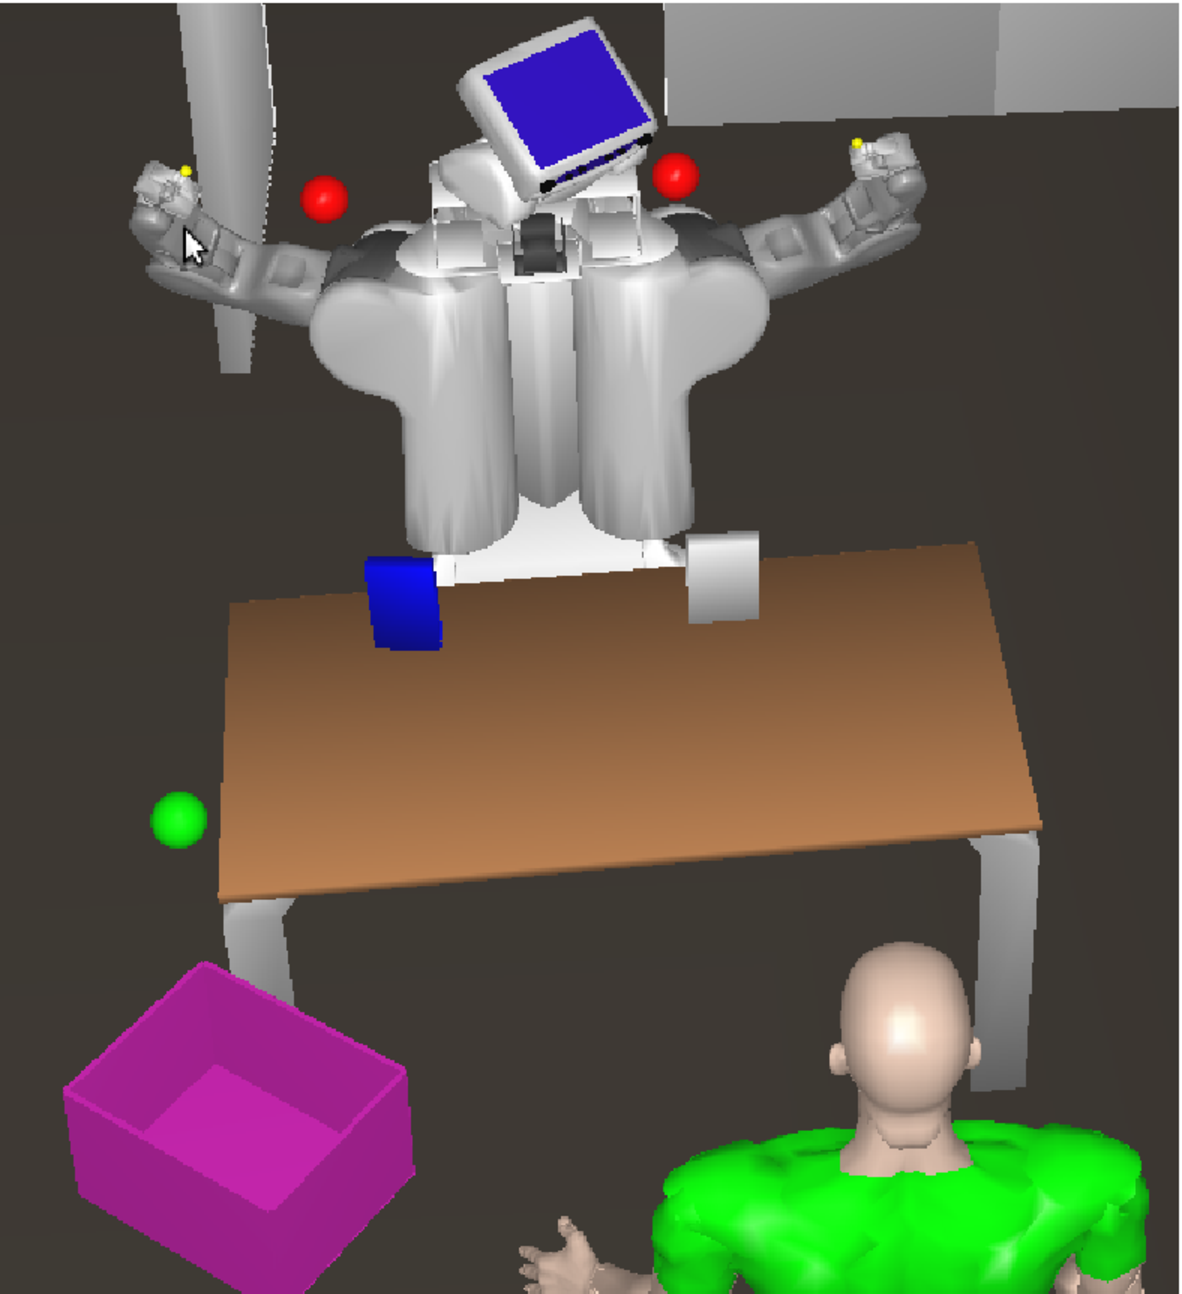
\includegraphics[scale=0.25]{img/case_study/helper/scenario2.pdf}
   }
  \subfigure {
    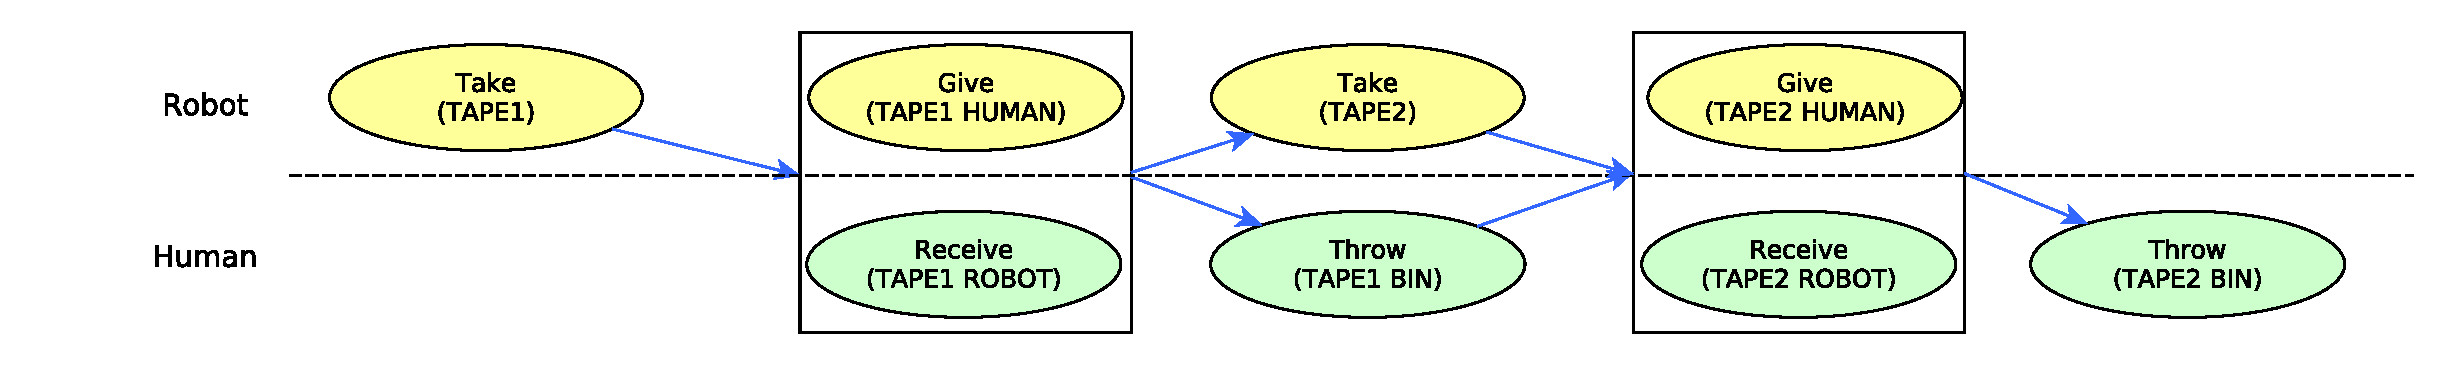
\includegraphics[scale=0.4]{img/case_study/helper/plan2.pdf}
  }
  \label{fig:case_study-helper_scenario2}
\end{figure}

While the robot is taking the \textit{TAPE1} the human moves
to take the \textit{TAPE2}. This deviates from the robot plan, so it
switches to the 'equal partners' modality, communicating the change to\
the user. The user throws the \textit{TAPE2} in the \textit{BIN} while
the robot takes the \textit{TAPE1} and handles it to the user. The user
takes the \textit{TAPE1} and throws it in the \textit{BIN}, completing the task.

In the second run the current modality is \textit{Human Leader} mode. The user is
asked to clean the table as he wishes. The user asks the robot to take
each tape and give it to him, throwing them in the trashbin.

\item
\textbf{Replanning after failed action}: 
In this scenario (figure \ref{fig:case_study-helper-scenario3}) the robot is the only agent able to reach the
bin, while both agents can reach the two tapes. The
robot is in \textit{Robot Leader} modality and, after examining the
environment, produces a plan.

\begin{figure}
  \caption[Robot helper experiment 3]{Replanning after failed action. Here we can see a first
    plan, produced at the start of the scenario, and a second,
    produced after the robot fails to take the \textit{TAPE2}. }
  \centering
  \subfigure{
    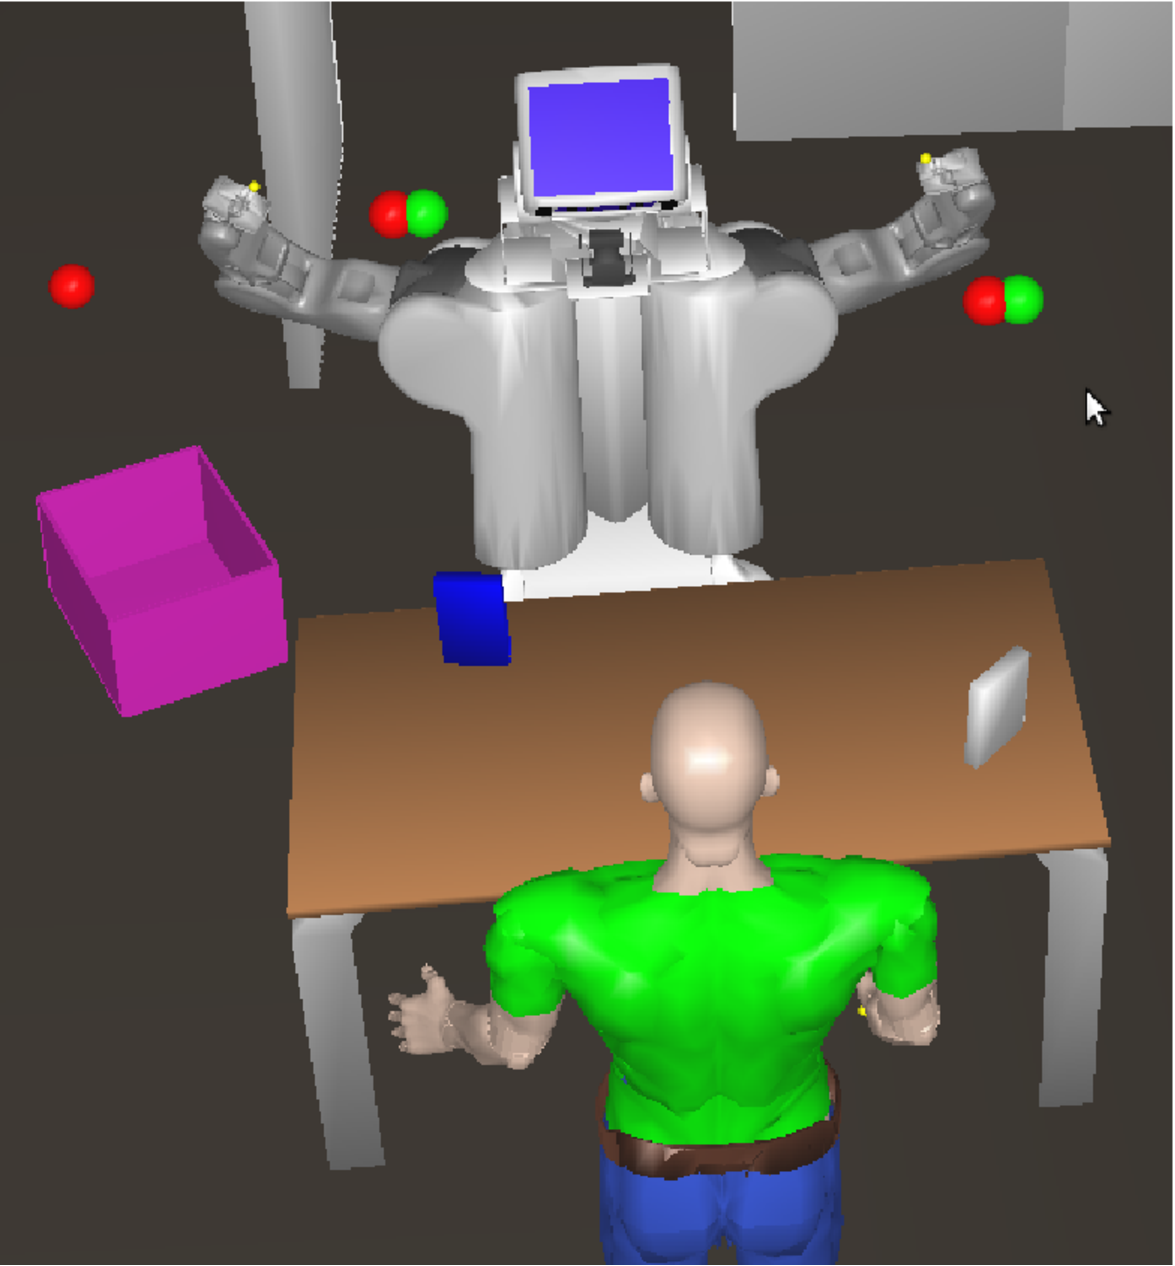
\includegraphics[scale=0.25]{img/case_study/helper/scenario3.pdf}
    }
    \subfigure {
      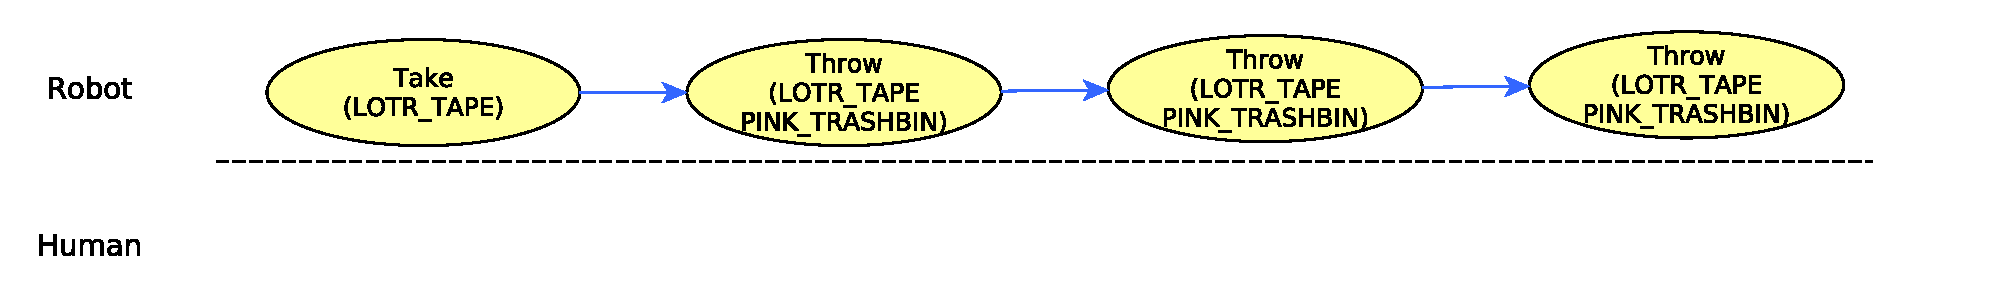
\includegraphics[scale=0.5]{img/case_study/helper/plan3.pdf}

      }
      \subfigure {
        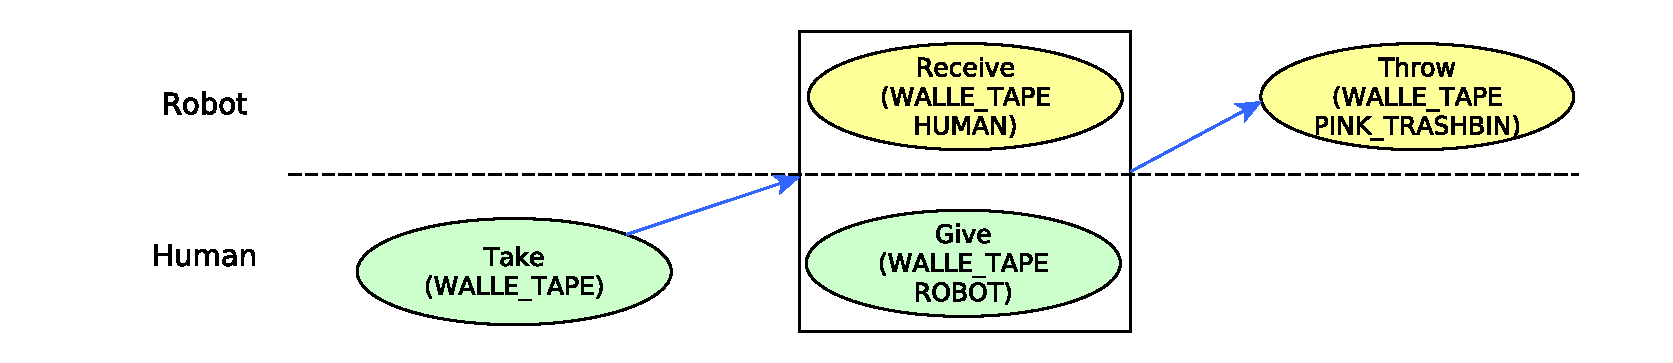
\includegraphics[scale=0.5]{img/case_study/helper/plan4.pdf}
      }
  \label{fig:case_study-helper-scenario3}
\end{figure}


After taking and throwing the \textit{TAPE1}, the robot tries to take the
\textit{TAPE2}, but fails because it is too far. The robot informs the user
and replans. The agents execute the plan, completing the task.

\item
\textbf{Replanning after human inactivity}.
In this run the robot computes that the \textit{TAPE3} and \textit{BIN}
are reachable only by the human, while the \textit{TAPE2} is reachable only by the robot. The robot computes a plan
and starts executing it, observing the human reactions. 
 After an initial stage when the human is
commited to the task, he does not execute a part of the plan (taking
the final tape and throwing it), so the robot looks for another
plan. The only solution to the problem is the one already computed at
the beginning, so the robot decides to ask
 the human to take the tape and throw it. A run of this
scenario is shown in figure ~\ref{fig:case_study-helper-experiment}. 
\end{itemize}

 
\begin{figure}
  \caption[Robot helper experiment 4]{The picture shows a run of our \textit{replanning after human
    inactivity scenario}. The different
    rows show, starting from top to bottom: the real world picture,
    the world state representation built by the robot, symbolic facts
    introduced in the knowledge base at each time step, action taken by the
    agents at each time step, the current plan calculated by the robot.}
  \centering
  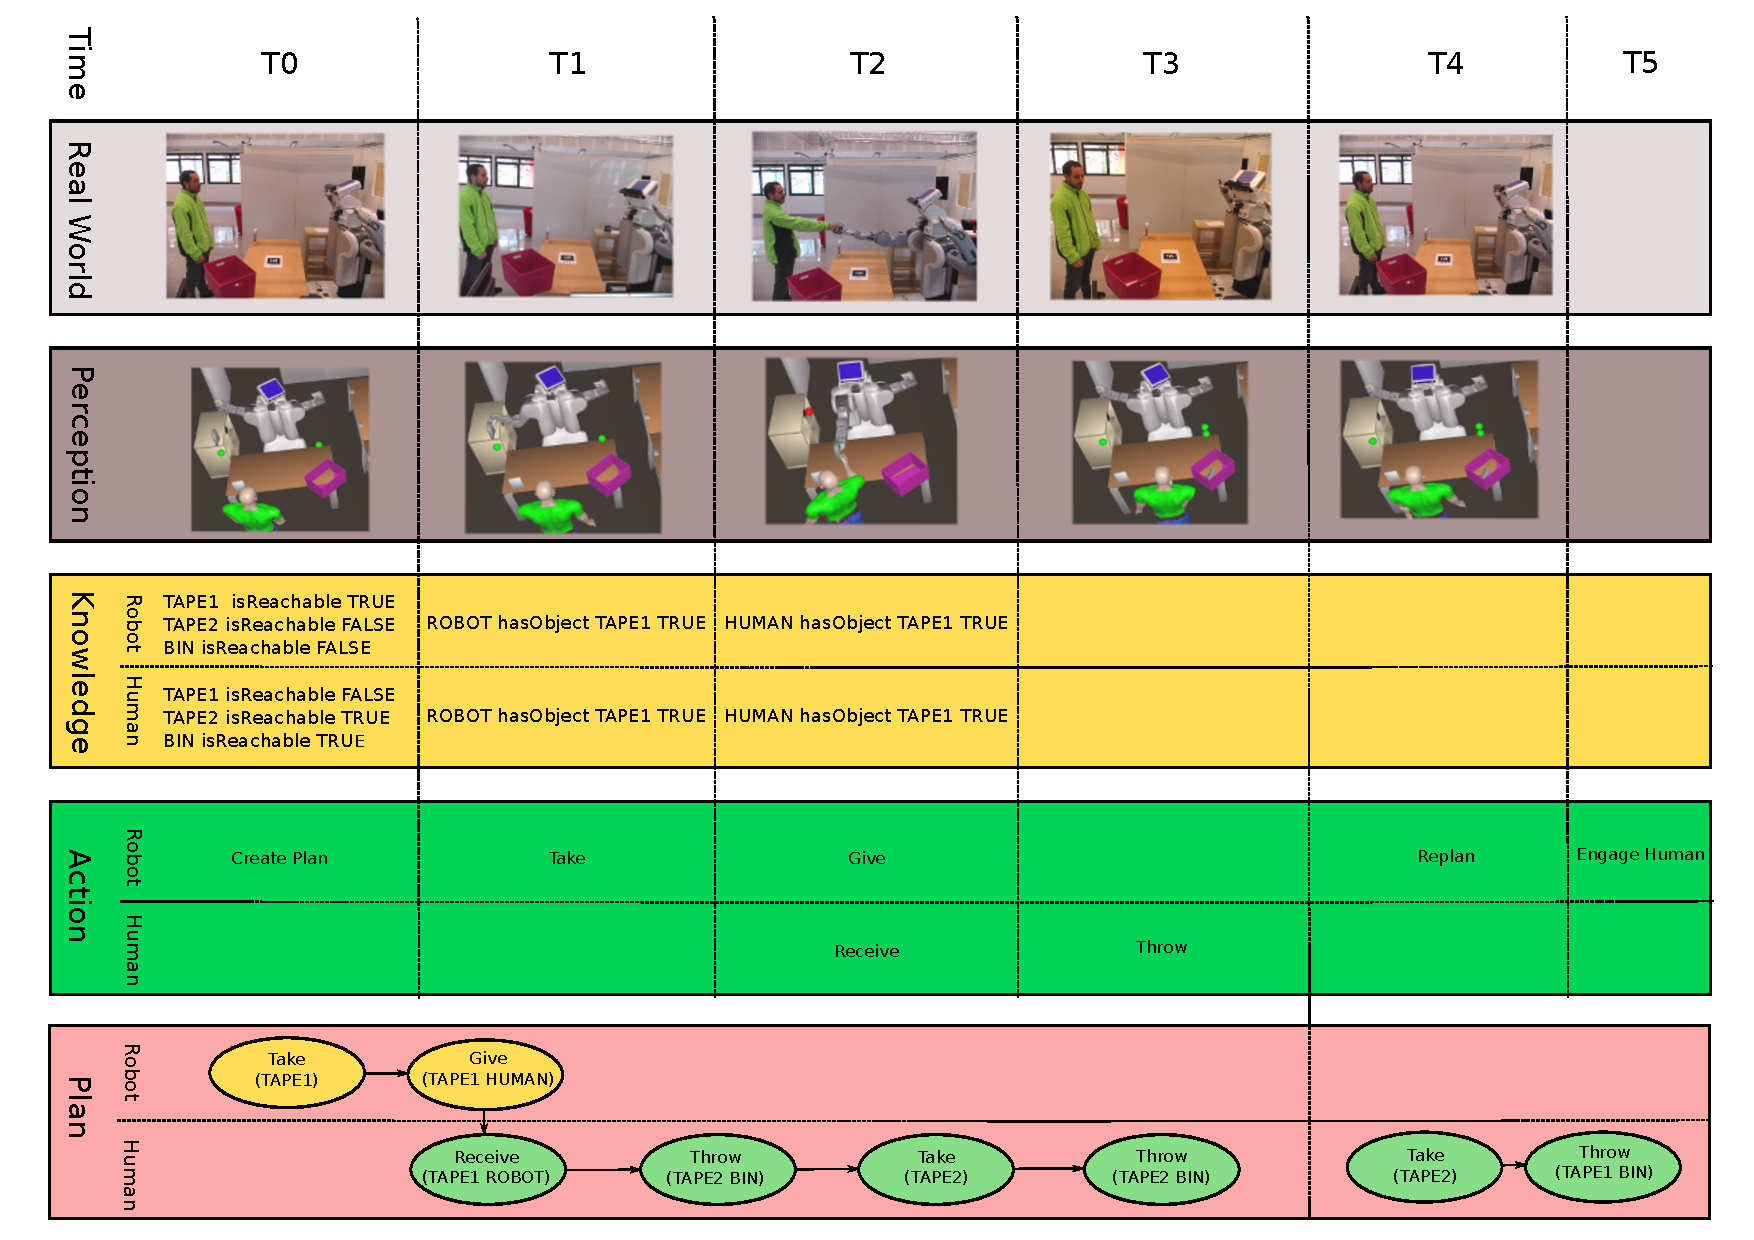
\includegraphics[angle=90, scale=0.7]{img/case_study/helper/complete_plan.pdf}
  \label{fig:case_study-helper-experiment}

\end {figure}


\subsection{Discussion}
\label{subsec:case_study-helper-discussion}
We review some of the main results of our experiments in this scenario:
\begin{itemize}

\item
\textbf{The system is able to handle joint goals}.
The system is able to create shared plans with different users, taking
into account the capabilities of each agent. When unexpected changes
in the world or task status arise, the system is able to quickly
replan, adapting to new scenarios. The system is able to execute this
joint goal in a human aware way. 
                                
\item
\textbf{The system is able to handle joint actions}.
The system is able to estimate user intentions in collaborative tasks and to choose appropriate actions, using a set of MOMDP models.

\item
\textbf{The system is able to handle user preferences}.
The system is able to adapt itself to user preferences, allowing the
human partner to give commands or to be more passive in its role and
switching from one modality to the other. 
\item
\textbf{The system is able to handle each agent beliefs}.
The system is able to represent different belief states for different agents and to take into accout what users can see, reach and know when creating a plan.

\item
\textbf{The system is able to monitor human actions}.
The system was able to understand when the human performed action such as taking or throwing objects.
\end{itemize}

